Nachdem nun die formalen Grundlagen gelegt sind, werden in diesem Abschnitt Grundbegriffe eingeführt, die notwendig für das Verständnis der nächsten Kapitel sind. Besonders wichtig sind insbesondere die Begriffe \enquote{Thread}, \enquote{Nebenläufigkeit} und \enquote{Wettkampfbedingung}, da diese Begriffe in der Arbeit intensiv behandelt werden.


\subsubsection{Definition von Thread}
Um definieren zu können, was ein Thread ist, müssen zuerst einige weitere Grundbegriffe eingeführt werden. 

Als \gls{Programm} wird in dieser Arbeit die konkrete Niederschrift eines Algorithmus bezeichnet. Die Elemente, aus denen das \gls{Programm} besteht, werden als \glspl{Anweisung} bezeichnet. Bei der Ausführung eines \glsuseri{Programm} werden Einzelschritte durchlaufen, diese bezeichnet man als \glspl{Aktivitaet}. Eine Sequenz von \glspl{Aktivitaet}, die ein isoliertes Problem abarbeitet, wird \emph{Prozess} genannt. Um diese Definition des Prozessbegriffs von späteren Definitionen abzugrenzen wird er im Folgenden \gls{Rechenprozess} genannt. Die Ausführungseinheit, auf der die Schritte eines \glsuseri{Rechenprozess} durchgeführt werden, wird \emph{Prozessor} genannt~\cite[S.~22]{Herrtwich1989}. In der Regel besitzt ein Rechner, beispielsweise ein PC, mehrere Ausführungseinheiten. Bei PCs gibt es eine Recheneinheit, die üblicherweise die meisten \glspl{Rechenprozess} ausführt und andere Prozessoren koordiniert, den \ac{cpu}.

Wenn ein \gls{Programm} auf einem Betriebssystem ausgeführt wird, erzeugt das Betriebssystem einen isolierten Adressraum, in dem das \gls{Programm} ausgeführt wird. Ein \gls{Rechenprozess}, der auf diese Weise ausgeführt wird, wird in dieser Arbeit als \emph{(System-)Prozess} bezeichnet. \textcite[Kapitel~2]{Tanenbaum2016} liefern eine gute Übersicht über Systemprozesse, dort als Prozesse bezeichnet. Systemprozesse können selbst weitere Systemprozesse starten, wenn das Betriebssystem dies zulässt. Diese Systemprozesse besitzen dann ihren eigenen Adressraum. Die Anzahl der Systemprozesse, die auf einem Rechner laufen, ist meist höher als die Anzahl der Prozessoren des Rechners. Somit können nicht alle Prozesse zur gleichen Zeit laufen. Damit dennoch alle Prozesse voranschreiten können, wechseln moderne Betriebssysteme die Systemprozesse, die auf den Prozessoren des Rechners ausgeführt werden, in schneller Folge. Dabei muss das Betriebssystem einige zu den Systemprozessen gehörende Daten, den \emph{Prozesskontrollblock}, tauschen, sodass der jeweils gerade ausführende Systemprozess seinen eigenen Prozesskontrollblock zur Verfügung hat. Dieser Tausch wird \emph{Kontextwechsel} genannt~\cite[S.~59]{Tanenbaum2016}.

Das Speichern und Laden der Prozesskontrollblöcken im Rahmen der Kontextwechsel von Systemprozessen benötigt eine nicht zu vernachlässigende Menge an Zeit. Ein solcher Zeitverbrauch wird auch als \emph{Overhead} bezeichnet. Um den Overhead von Kontextwechseln zu vermindern, bieten moderne Betriebssysteme Systemprozessen die Möglichkeit \glspl{Rechenprozess} zu erzeugen, die denselben Adressraum wie der erzeugende Systemprozess besitzen. Ein auf diese Art erzeugter \gls{Rechenprozess} heißt \emph{Thread}. Da die Menge der thread-eigenen Daten, des \emph{Threadkontrollblocks}, deutlich geringer ist als die des Prozesskontrollblocks, erzeugt der Kontextwechsel zwischen Threads einen geringeren Overhead. Zudem können Threads aufgrund des gemeinsamen Adressraums einfacher auf geteilte Ressourcen zugreifen. Das vereinfacht die Kooperation zwischen diesen \glsuserii{Rechenprozess}~\cite[S.~139~ff.]{Tanenbaum2016}.

\paragraph{Anweisungen und Petri-Netze}
Um formal Eigenschaften eines \glsuseri{Programm} zu beschreiben, ist es möglich dieses mittels eines Petri-Netzes (automatisiert) zu modellieren. Dazu müssen Petri-Netz-Konstrukte genutzt werden, die die \glspl{Anweisung} des \glsuseri{Programm} abbilden können. Für die Analyse nebenläufiger \glspl{Programm} sind nur sogenannte \emph{Rendezvous}-\glspl{Anweisung} sowie Kontrollstrukturen relevant~\cite{Goel1990}. Für diese lassen sich Unter-Petri-Netze definieren, die deren Verhalten modellieren. Da die Modellierung von Verzweigungen durch Unter-Petri-Netze in \cite[Abbildung 3.1]{Goel1990} semantisch nicht ganz korrekt ist, wird sie in Abbildung~\ref{fig:supnetifelse} korrigiert dargestellt. 
\begin{figure}
	\centering
	\begin{tikzpicture}[node distance=2cm,on grid, auto]
		\node[place, label=$p_1$] (p1) {};
		\node[transV, label=\texttt{if}, above right = of p1] (if) {};
		\node[transV, label=\texttt{else},below right = of p1] (else) {};
		\node[right = of if] (dots1){$\dots$};
		\node[right = of else] (dots2){$\dots$};
		\node[place, label=$p_2$, right = of dots1] (p2) {};
		\node[place, label=$p_3$, right = of dots2] (p3) {};
		\node[transV, label=$t_1$, right = of p2] (t1) {};
		\node[transV, label=$t_2$, right = of p3] (t2) {};
		\node[place, label=$p_4$, below right = of t1] (p4) {};
		\node[transV, label=\texttt{end if}, right = of p4] (endif) {};
	
	
	
		\draw 
		(p1) edge[post] (if)
		(p1) edge[post] (else)
		(if) edge[post] (dots1)
		(else) edge[post] (dots2)
		(dots1) edge[post] (p2) 
		(dots2) edge[post] (p3) 
		(p2) edge[post] (t1)
		(p3) edge[post] (t2)
		(t1) edge[post] (p4)
		(t2) edge[post] (p4)
		(p4) edge[post] (endif)
		;
	\end{tikzpicture}
	\caption[Semantisch korrigiertes Unter-Petri-Netz zu Modellierung von Verzweigungen.]{Semantisch korrigiertes Unter-Petri-Netz zu Modellierung von Verzweigungen nach \cite[Abbildung~3.1]{Goel1990}.}\label{fig:supnetifelse}
\end{figure}

Die Plätze $p_1,p_2,p_3,p_4$ und die Transitionen $t_1,t_2$ sind Hilfselemente die die semantische Korrektheit der Transitionen \code{if}, \code{else} und \code{end if} sicherstellen. Eine Markierung kann exklusiv nur von \code{if} oder von \code{else} zum Feuern verwendet werden. Durch die Transitionen $t_1$ und $t_2$ entsteht eine Markierung in $p_5$ wodurch \code{end if} feuern kann egal ob anfangs \code{if} oder \code{else} gefeuert hat. $p_2$ und $p_3$ existierten, damit das Petri-Netz ein bipartiter Graph bleibt, sich also immer Plätze und Transitionen \enquote{abwechseln}. Die Modellierung eines \code{switch}-Statements erfolgt analog, indem die Anzahl der Pfade zwischen $p_1$ und $p_4$ angepasst wird.

\subsubsection{Nebenläufigkeit}\label{sec:nebenl}
Im vorherigen Abschnitt wurde beschrieben, dass verschiedene \glspl{Rechenprozess} unabhängig von einander \enquote{gleichzeitig} ablaufen können. Ein \gls{Programm} wird häufig als \emph{Sequenz} von \glspl{Anweisung} verstanden. In der Definition von \gls{Programm} in dieser Arbeit wird bewusst auf das Wort Sequenz verzichtet, denn bei vielen \glsuserii{Programm} kann es bei bestimmten \glspl{Anweisung} irrelevant sein, in welcher Reihenfolge oder ob sie sogar gleichzeitig ausgeführt werden. Man betrachte das folgende \gls{Programm} in Listing~\ref{lst:squareSeqEx}, das die Quadratsumme zweier Ganzzahlen (im Folgenden auch Quadratsumme genannt) ausgibt.

\begin{lstlisting}[caption={[Beispiel eines \glsentryuseri{Programm} das sequentiell die Summe von Quadraten zweier Ganzzahlen berechnet.]Beispiel eines \glsuseri{Programm} das die Summe von Quadraten zweier Ganzzahlen berechnet. Die Berechnung der Quadratzahlen wird nacheinander in einer fest definierten Sequenz durchgeführt.}, label={lst:squareSeqEx},float={!htbp}]
printSummedSquare(int a, int b){
  x <- a*a (*\label{lst:squareSeqEx:aa}*)
  y <- b*b (*\label{lst:squareSeqEx:bb}*)
  print(x+y) (*\label{lst:squareSeqEx:print}*)
}
\end{lstlisting}
Es ist leicht zu erkennen, dass es vollkommen egal ist, ob zuerst \code{x} oder \code{y} ausgerechnet wird oder die Berechnungen simultan stattfinden. Einzig der Ausgabebefehl in Zeile~\ref{lst:squareSeqEx:print} muss ausgeführt werden, nachdem \code{x} und \code{y} berechnet wurden. Zuzulassen, dass die Ausführreihenfolge in dem \gls{Programm} nicht definiert ist, bringt das Design des \glsuseri{Programm} näher an die Problembeschreibung \enquote{gib die Quadratsumme zweier Ganzzahlen aus} und ermöglicht auch eine potenziell schnellere Berechnung, da die Quadrate gleichzeitig berechnet werden können.

Paare oder Gruppen von \glspl{Anweisung}, die gleichzeitig oder in beliebiger Reihenfolge ausgeführt werden, heißen \emph{nebenläufig}. Da die Ausführungsreihenfolge der Anweisungen in Zeile~\ref{lst:squareSeqEx:aa} und Zeile~\ref{lst:squareSeqEx:bb} egal ist, könnten diese Anweisungen auch nebenläufig definiert werden.

Eine der obigen Problemstellung nähere Implementierung der Quadratsumme könnte unter Nutzung von Nebenläufigkeit wie Listing~\ref{lst:squareConcEx} aussehen, dabei wird auf die Schreibweise von \textcite[S.~16]{Herrtwich1989} zurückgegriffen:
\begin{lstlisting}[caption={[Beispiel eines \glsuseri{Programm} mit nebenläufigem Code in einem \code{conc}-Block.]Beispiel eines \glsuseri{Programm} mit nebenläufigem Code in einem \code{conc}-Block. Das \gls{Programm} gibt die Summe von zwei Quadratzahlen aus, wobei die Berechnung der Quadratzahlen nebenläufig stattfindet.}, label={lst:squareConcEx},float={!htbp}]
printSummedSquare(int a, int b){
  conc 
    x <- a*a ||
    y <- b*b
  conc end
  print(x+y)
}
\end{lstlisting}
In einem \code{conc}-Block, definiert durch \code{conc} und \code{conc end}, sind alle \glspl{Anweisung} die durch \code{||} getrennt sind als nebenläufig zu verstehen. Wie man an obigem Beispiel erkennen kann, beschäftigt Nebenläufigkeit sich besonders mit der Struktur und der Möglichkeit der Zusammensetzung voneinander unabhängiger \glspl{Anweisung}. Somit ist es Aufgabe der nebenläufigen Programmierung, Probleme oder Aufgaben in unabhängige Teile zu zerlegen und zu strukturieren~\cite{Pike2012,Hettel2016}. Blöcke von \glspl{Anweisung}, die (bezüglich der Aufgabe) nebenläufig sein könnten, aber als Anweisungssequenz definiert sind (siehe Listing~\ref{lst:squareSeqEx} Zeile 2 und 3), werden in dieser Arbeit als \emph{pseudo-sequentialisiert} bezeichnet.

Bei der Definition nebenläufiger Anweisungen ist allerdings Vorsicht geboten, da sichergestellt werden muss, dass zwei Anweisungen auch tatsächlich nebenläufig sein dürfen. Eine \gls{Anweisung} kann beispielsweise durch einen Compiler in mehrere \glspl{Anweisung} geteilt werden oder schon aus mehreren \glspl{Anweisung} bestehen (man denke zum Beispiel an Funktionsaufrufe). Solche \glspl{Anweisung} werden \gls{nichtAtomar} genannt. Eine Menge von nebenläufigen \glspl{Anweisung}, von denen mindestens eine \gls{nichtAtomar} ist, kann \emph{verzahnt} ausgeführt werden. Eine Ausführung von \glspl{Anweisung} ist verzahnt, wenn zwischen der Ausführung der Teile einer \glsuseri{nichtAtomar} \gls{Anweisung} andere \glspl{Anweisung} ausgeführt werden. Abbildung \ref{fig:concAnweisungen} zeigt zur Veranschaulichung die verschiedenen Möglichkeiten, wie zwei nebenläufige \glspl{nichtAtomar} \glspl{Anweisung} im Zeitverlauf ausgeführt werden können, sowohl auf einem Prozessor als auch auf zwei Prozessoren. Dadurch kann es passieren, dass Anweisungen, die zuerst den Anschein haben, nebenläufig sein zu können, nicht nebenläufig sein dürfen, weil eine verzahnte Ausführung der zugehörigen Aktivitäten ein unerwünschtes Ergebnis liefern würde. 

\begin{figure}[hbt]
	\centering
\newlength\aOne
\newlength\aTwo
\newlength\aThree
\newlength\bOne
\newlength\bTwo
\pgfmathsetlength{\aOne}{4cm}
\pgfmathsetlength{\aTwo}{2cm}
\pgfmathsetlength{\aThree}{3cm}
\pgfmathsetlength{\bOne}{2.5cm}
\pgfmathsetlength{\bTwo}{3.7cm}
\begin{subfigure}{\textwidth}
	\centering
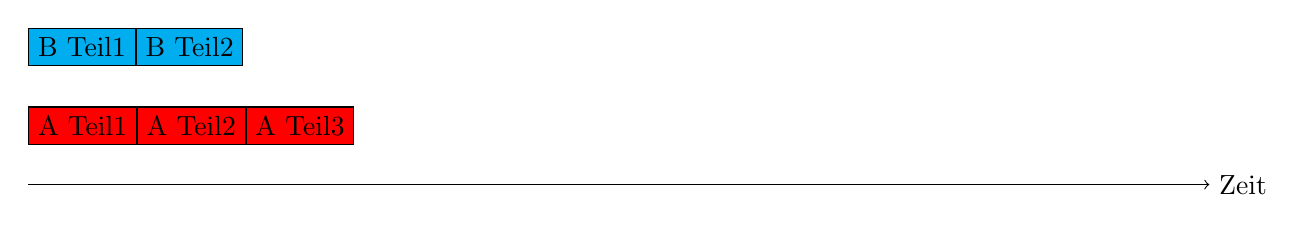
\begin{tikzpicture}

	\draw[->] (0,0) -- (15,0) node[right] {Zeit};
	
	\node[draw,fill=red, anchor=south west, minimum width = \aOne] at (0, .5) (A1) {A Teil1};
	\node[draw,fill=red, anchor=west, minimum width = \aTwo] at (A1.east) (A2) {A Teil2};
	\node[draw,fill=red, anchor=west, minimum width = \aThree] at (A2.east) (A3) {A Teil3};
	
	\node[draw,fill=cyan, anchor=south west, minimum width = \bOne] at (0, 1.5) (B1) {B Teil1};
	\node[draw,fill=cyan, anchor=west, minimum width = \bTwo] at (B1.east) (B2) {B Teil2};

\end{tikzpicture}
\subcaption{Gleichzeitige Ausführung der \glspl{Anweisung} A und B auf zwei Prozessoren}
\end{subfigure}
\\[1.5em]
\begin{subfigure}{\textwidth}
	\centering
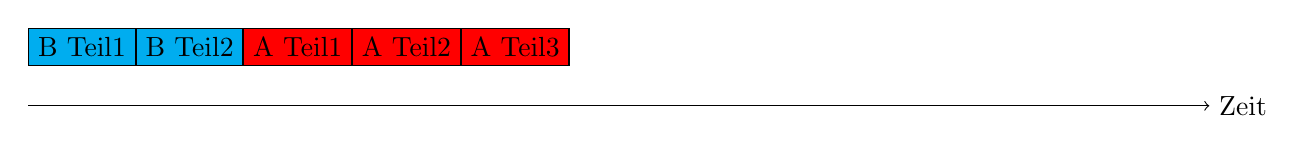
\begin{tikzpicture}

	\draw[->] (0,0) -- (15,0) node[right] {Zeit};
	
	\node[draw,fill=cyan, anchor=south west, minimum width = \bOne] at (0, .5) (B1) {B Teil1};
	\node[draw,fill=cyan, anchor=west, minimum width = \bTwo] at (B1.east) (B2) {B Teil2};
	\node[draw,fill=red, anchor=west, minimum width = \aOne] at (B2.east) (A1) {A Teil1};
	\node[draw,fill=red, anchor=west, minimum width = \aTwo] at (A1.east) (A2) {A Teil2};
	\node[draw,fill=red, anchor=west, minimum width = \aThree] at (A2.east) (A3) {A Teil3};
\end{tikzpicture}
\subcaption{Sequenzielle Ausführung der \glspl{Anweisung} A und B auf einem Prozessor}
\end{subfigure}
\\[1.5em]
\begin{subfigure}{\textwidth}
	\centering
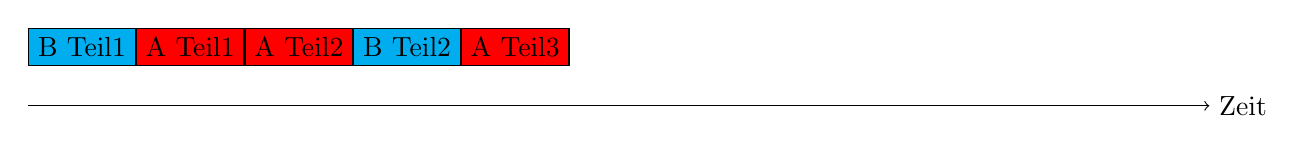
\begin{tikzpicture}

	\draw[->] (0,0) -- (15,0) node[right] {Zeit};
	
	\node[draw,fill=cyan, anchor=south west, minimum width = \bOne] at (0, .5) (B1) {B Teil1};
	\node[draw,fill=red, anchor=west, minimum width = \aOne] at (B1.east) (A1) {A Teil1};
	\node[draw,fill=red, anchor=west, minimum width = \aTwo] at (A1.east) (A2) {A Teil2};
	\node[draw,fill=cyan, anchor=west, minimum width = \bTwo] at (A2.east) (B2) {B Teil2};
	\node[draw,fill=red, anchor=west, minimum width = \aThree] at (B2.east) (A3) {A Teil3};

\end{tikzpicture}
\subcaption{Verzahnte Ausführung der \glspl{Anweisung} A und B auf einem Prozessor}
\end{subfigure}

\caption[Mögliche Ausführungen nebenläufiger \glsentryplural{Anweisung}.]{Mögliche Ausführungen nebenläufiger \glspl{Anweisung}. Die Grafik bildet eine Abbildung aus \cite{Herrtwich1989} nach.}\label{fig:concAnweisungen}
\end{figure}

Werden nebenläufige \glspl{Anweisung} parallel ausgeführt, spricht man auch von \emph{Multiprocessing}. Handelt es sich bei den Prozessen um Threads, wird der Begriff \emph{Multithreading} genutzt.

\paragraph{Nebenläufigkeit und Petri-Netze}
Um ein eindeutiges Verständnis des hier genutzten Begriffs der Nebenläufigkeit zu geben, wird dieser auch in Bezug auf Petri-Netze definiert. Wichtig anzumerken ist, dass der hier beschriebene Begriff vom üblichen Verständnis der Nebenläufigkeit in Petri-Netzen abweicht. 

Normalerweise werden Petri-Netze  als inhärent nebenläufig verstanden, da durch die Transitionsregel zu jeder Zeit jede beliebige Transition feuern kann, deren Vorbedingungen  erfüllt sind. Der hier verwendete Begriff bezieht sich allerdings darauf, dass \glspl{Anweisung} unabhängig voneinander, ohne sich gegenseitig zu beeinflussen, ausführbar sind. Das Feuern einer Transition kann aber den Vorbereich einer anderen Transition verändern, wodurch sie beeinflusst wird.

In dieser Arbeit heißen zwei Transitionen $t_1, t_2$ eines Petri-Netzes $N$ genau dann nebenläufig, wenn ${}^\circ t_1 \cap {}^\circ t_2 = \emptyset$ gilt und eine Markierung $m_\text{conc}$ im Erreichbarkeitsgraphen $\E{N}$ existiert, in der sowohl $t_1$ als auch $t_2$ aktiviert sind.

\subsubsection{Folgen von Nebenläufigkeit}\label{sec:nebenl-folgen}
Wie in Abschnitt \ref{sec:nebenl} beschrieben, muss ein \gls{Programm} keine Sequenz von \glspl{Anweisung} sein, sondern kann auch nebenläufige \glspl{Anweisung} enthalten. Diese Möglichkeit hat eine Reihe von Folgen, die es bei der nebenläufigen Programmierung zu beachten gilt.
\paragraph{Nichtdeterminismus}
Enthält ein \gls{Programm} nebenläufige \glspl{Anweisung}, ist die Reihenfolge der daraus resultierenden \glspl{Aktivitaet} nicht definiert und kann sich bei jedem Programmdurchlauf ändern. Die Ausführung ist also \emph{nichtdeterministisch}, als direkte Folge der Nebenläufigkeit~\cite[S.~17~f.]{Herrtwich1989}. Erwartet man von einem \gls{Programm} \emph{Determiniertheit}\footnote{Es kann durchaus sein, dass Determiniertheit in einem \gls{Programm} nicht gewünscht ist. Man betrachte beispielsweise ein \gls{Programm}, das einen echten Zufallsgenerator beschreibt. Hier wäre Determiniertheit ein direkter Widerspruch zur Aufgabe des \glsuseri{Programm}.}, also die Eigenschaft, dass gleiche Eingaben immer zu den gleichen Ausgaben führen, ist Nichtdeterminismus in der Regel zu vermeiden. Liefert ein \gls{Programm} bei jeder beliebigen Ausführreihenfolge dasselbe Ergebnis, ist es trotz Nichtdeterminismus weiterhin determiniert, weil die Ausführreihenfolge für das Ergebnis keine Rolle spielt~\cite[S.~18~f.]{Herrtwich1989}. 
\paragraph{Nichtreproduzierbarkeit}
Da das Wissen und die Kontrolle über die Ausführreihenfolge abgegeben wird, wird die Nachvollziehbarkeit des Programmablaufs erschwert~\cite[S.~20]{Herrtwich1989}. Tritt beispielsweise ein Fehler auf, kann im Nachhinein nicht ermittelt werden was die Ausführreihenfolge war, die zu dem Fehler geführt hat. Dasselbe Problem ergibt sich ebenfalls, wenn ein nichtdeterminiertes \gls{Programm} eine Lösung ausgibt und nachvollzogen werden soll, welche Ausführreihenfolge zu diesem Ergebnis geführt hat. Insbesondere das Testen von Software wird dadurch erschwert, da es unmöglich ist bei jedem Test dieselben Bedingungen herzustellen, sodass beispielsweise Tests Fehler nicht verlässlich aufzeigen, weil diese nur bei bestimmten Ausführreihenfolgen auftreten~\cite[S.~20]{Herrtwich1989}. Somit muss ein Test entweder alle möglichen Ausführreihenfolgen simulieren oder es muss anderweitig sichergestellt werden, dass die Ausführreihenfolge der nebenläufigen \glspl{Anweisung} keine Rolle spielt.
\paragraph{Wettkampfbedingungen}
Ressourcen (zum Beispiel Drucker, Variablen und Dateien) und insbesondere Daten spielen in \glsuserii{Programm} eine zentrale Rolle. Greift eine Gruppe von nebenläufigen \glspl{Anweisung} auf dieselben (geteilten) Daten zu, ist die Reihenfolge des Zugriffs, wie alle anderen \glspl{Aktivitaet}, beliebig. Wenn mindestens eine der \glspl{Anweisung} schreibend auf die geteilten Daten zugreift (diese also verändert), hängt der Zustand der Ausgabe des \glsuseri{Programm} im Allgemeinen von der Reihenfolge der Ausführung ab. Diese Situation wird \emph{Wettkampfbedingung} (engl. Race Condition) genannt~\cite{Hettel2016}. 

Erwähnenswert ist hier, dass Wettkampfbedingungen nur auftreten können, wenn die geteilten Daten nebenläufig \emph{geändert} werden. Ausschließlich lesende Zugriffe sind unkritisch, da die Daten unabhängig von der Ausführreihenfolge immer identisch sind. Wenn Daten von lesenden \glspl{Anweisung} zu jederzeit in einem Zustand gefunden werden, der korrekt ist, werden sie als \emph{threadsicher} bezeichnet.

Formal können Wettkampfbedingungen auch mittels erweiterten Petri-Netzen definiert werden. Dazu betrachtet man, ob Variablen des erweiterten Petri-Netzes sich in den Lese- und Schreibmengen von nebenläufigen Transitionen überschneiden. Diese Variablen werden \emph{kritische} Variablen genannt. Die Menge der kritischen Variablen, die zur Existenz von Wettkampfbedingungen führen, ist gegeben durch
\begin{align*}
	V_\text{krit} = \;\bigcup_{\mathclap{\substack{s,t\, \in T\\s, t \text{ nebenläufig}}}} \;\left( \strut{S(s) \cap (S(t) \cup L(t))}\right).
\end{align*}

Ein Paar von Transitionen $(t_1, t_2)$ eines erweiterten Petri-Netzes \emph{erzeugt} eine Wettkampfbedingung, wenn die Transitionen dazu führen, dass eine Variable in die Menge der kritischen Variablen aufgenommen wird. Eine Markierung $m$ des Erreichbarkeitsgraphen $\E{N}$ eines Petri-Netzes $N$ enthält eine Wettkampfbedingung, wenn ein Paar von Transitionen $(t_1, t_2)$ existiert, das eine Wettkampfbedingung erzeugt, und $t_1$ und $t_2$ in $m$ aktiviert sind.

\begin{figure}
	\centering
	\begin{tikzpicture}[node distance=2cm,on grid, auto]
		\node[place, label=$p_1$] (p1) {};
		\node[transV, label=$t_1$, right = of p1] (t1) {};
		\node[place, label=$p_2$, tokens=1, above right = of t1] (p2) {};
		\node[place, label=$p_3$, tokens=1, below right = of t1] (p3) {};
		\node[transV,label=$t_2$, right = of p2,label=below:{\LSset{a,{\color{red}b}}{a}} ] (t2){};
		\node[transV,label=$t_3$, right = of p3,label=below:{\LSset{b}{{\color{red}b}}}] (t3){};
		\node[place, label=$p_4$, right = of t2] (p4) {};
		\node[place, label=$p_5$, right = of t3] (p5) {};
		\node[transV, label=$t_4$, below right = of p4] (t4) {};
		\node[place, label=$p_6$, right = of t4] (p6) {};
	
	
	
		\draw 
		(p1) edge[post] (t1)
		(t1) edge[post] (p2)
		(t1) edge[post] (p3)
		(p2) edge[post] (t2)
		(p3) edge[post] (t3)
		(t2) edge[post] (p4)
		(t3) edge[post] (p5)
		(p4) edge[post] (t4)
		(p5) edge[post] (t4)
		(t4) edge[post] (p6)
		;
	\end{tikzpicture}
	\caption[Ein erweitertes Petri-Netz, dessen Markierung eine Wettkampfbedingung enthält.]{Ein erweitertes Petri-Netz, dessen Markierung eine Wettkampfbedingung enthält. Die Schreibmenge von $t_3$ enthält die Variable $b$, diese ist allerdings auch in der Lesemenge von $t_2$ enthalten. Die problematische Variable {\color{red}$b$} ist rot markiert. Das Auftauchen von $b$ in der Lesemenge von $t_3$ stellt kein Problem dar.}\label{fig:wettkampfpetri}
\end{figure}

Um das Konzept zu veranschaulichen, ist in Abbildung~\ref{fig:wettkampfpetri} ein erweitertes Petri-Netz gezeigt, dessen Markierung eine Wettkampfbedingung enthält. Die Plätze $p_2$ und $p_3$ enthalten je eine Markierung. Daher müssen nun die Transitionen betrachtet werden, die aktiviert sind. Diese sind $\{t_2,t_3\}$. Wie in der Abbildung rot markiert, ist ersichtlich, dass sich die Lese- und Schreibmenge der Transitionen überschneiden, da $V_\text{krit} = \{b\} \neq \emptyset$ ist. Somit enthält die gezeigte Markierung eine Wettkampfbedingung.

Ein erweitertes Petri-Netz enthält eine Wettkampfbedingung, wenn mindestens eine Markierung seines Erreichbarkeitsgraphen eine Wettkampfbedingung enthält.

Aufgabe der nebenläufigen Programmierung ist es also, \glspl{Anweisung} so zu strukturieren, dass alle von nebenläufigen \glspl{Anweisung} genutzten Daten threadsicher sind oder Daten, die nicht threadsicher sind, explizit synchronisiert werden. Über die Modellierung von Petri-Netzen ausgedrückt, gilt es also die Struktur eines \glsuseri{Programm} so zu definieren, dass in dem Petri-Netz, welches das \gls{Programm} modelliert, keine Wettkampfbedingungen existieren.

\subsubsection{Synchronisierung}
Um das Auftreten von Wettkampfbedingungen beim schreibenden Zugriff von nebenläufigen \glspl{Anweisung} auf geteilte Ressourcen zu vermeiden, muss sichergestellt werden, dass der Endzustand nach der Ausführung der \glspl{Anweisung} unabhängig von der Ausführreihenfolge der daraus resultierenden \glspl{Aktivitaet} ist. Dieser Vorgang wird \emph{Synchronisierung} genannt~\cite[S.~4]{Maurer2019}.

\paragraph{Synchronisierungsanforderungen} Nach \textcite[S.~132~ff.]{Herrtwich1989} gibt es allgemein zwei Arten von Anforderungen an Synchronisierungsmechanismen, je nachdem welche Art von Zugriff auf geteilte Ressourcen stattfindet. Sie unterscheiden dabei zwischen \emph{kausal abhängigen} Relationen und \emph{kausal unabhängigen} Relationen zwischen nebenläufigen \glspl{Anweisung}. Ist \gls{Anweisung} $B$ kausal abhängig von \gls{Anweisung} $A$, so dürfen die \glspl{Aktivitaet} von $B$ erst ausgeführt werden, nachdem die \glspl{Aktivitaet} von $A$ abgeschlossen sind. Beispielsweise werden in der Blocklib Chunks im Hintergrund geladen. Benötigt eine \gls{Anweisung} eines Spielelements einen noch nicht geladenen Chunk, so muss die Ausführung der zugehörigen \gls{Aktivitaet} solange aufgeschoben werden, bis der Chunk geladen ist. Bei kausal unabhängigen Relationen muss sichergestellt werden, dass der Zugriff auf die Ressourcen nicht zur gleichen Zeit stattfindet.  Beispielsweise wird die Liste der zu zeichnenden Objekte in der Blocklib von verschiedenen Systemen angepasst. Hier muss also darauf geachtet werden, dass diese Anpassungen zeitlich getrennt stattfinden. Sonst könnten beispielsweise hinzugefügte Elemente verloren gehen könnten, wenn zwei Threads parallel Elemente hinzufügen, weil einer die Änderungen des anderen überschreibt.

\paragraph{Synchronisierungsmethoden} Es gibt mehrere Möglichkeiten, die Synchronisierung zwischen nebenläufigen \glspl{Anweisung} zu erreichen. \textcite{Michael1996} unterteilen Algorithmen diesbezüglich in zwei Kategorien: \emph{blockierende} und \emph{nicht-blockierende}. Blockierende Synchronisierungsalgorithmen definieren sogenannte \emph{kritische Bereiche}. Ein kritischer Bereich ist eine Menge von \glspl{Anweisung} von deren \glspl{Aktivitaet} nur eine gleichzeitig ausgeführt werden darf. Sind mehrere auszuführende \glspl{Aktivitaet} Teil eines kritischen Bereichs, muss durch \emph{Sperren} (engl. Locks) sichergestellt werden, dass nur eine der \glspl{Aktivitaet} gleichzeitig ausgeführt wird. Dadurch führen laut \textcite{Michael1996} solche Synchronisierungsmethoden möglicherweise dazu, dass \glspl{Rechenprozess} durch andere \glspl{Rechenprozess} beliebig lang beim Zugriff auf geteilte Daten aufhalten können.

Nicht-blockierende Algorithmen dagegen garantieren, dass mindestens einer der beteiligten \glspl{Rechenprozess} mit einer endlichen Anzahl an Schritten endet. Zudem konnte \textcite{Herlihy1991} bereits 1991 zeigen, dass beispielsweise unter Verwendung von atomaren \emph{Compare-and-Swap}-Instruktionen Datenstrukturen implementiert werden können, auf die nicht-blockierend von einer unbegrenzten Zahl an nebenläufigen \glspl{Aktivitaet} zugegriffen werden kann. Durch die Atomarität der genutzten \glspl{Anweisung} wird sichergestellt, dass die geteilten Ressourcen nicht in einen unvorhergesehenen Zustand übergehen. Die eben genannte Instruktion Compare-and-Swap ist eine \gls{Anweisung}, in der atomar der Wert einer Variable ausgelesen und mit einem übergebenen Wert verglichen wird (Compare). Danach wird, weiterhin atomar, der Inhalt Variable mit einem zweiten übergebenen Wert genau dann überschrieben (Swap), wenn die verglichenen Werte identisch waren. Die Instruktion gibt dann den vorherigen Wert zurück. Eine andere Variante der Instruktion gibt zurück, ob der Wert überschrieben wurde oder nicht. Die Atomarität dieser gesamten Instruktion muss durch die Hardware sichergestellt werden, das ist softwareseitig nicht möglich. Alle gängigen \acp{cpu} stellen Instruktionen dieser Art zur Verfügung.
